\documentclass[1p]{elsarticle_modified}
%\bibliographystyle{elsarticle-num}

%\usepackage[colorlinks]{hyperref}
%\usepackage{abbrmath_seonhwa} %\Abb, \Ascr, \Acal ,\Abf, \Afrak
\usepackage{amsfonts}
\usepackage{amssymb}
\usepackage{amsmath}
\usepackage{amsthm}
\usepackage{scalefnt}
\usepackage{amsbsy}
\usepackage{kotex}
\usepackage{caption}
\usepackage{subfig}
\usepackage{color}
\usepackage{graphicx}
\usepackage{xcolor} %% white, black, red, green, blue, cyan, magenta, yellow
\usepackage{float}
\usepackage{setspace}
\usepackage{hyperref}

\usepackage{tikz}
\usetikzlibrary{arrows}

\usepackage{multirow}
\usepackage{array} % fixed length table
\usepackage{hhline}

%%%%%%%%%%%%%%%%%%%%%
\makeatletter
\renewcommand*\env@matrix[1][\arraystretch]{%
	\edef\arraystretch{#1}%
	\hskip -\arraycolsep
	\let\@ifnextchar\new@ifnextchar
	\array{*\c@MaxMatrixCols c}}
\makeatother %https://tex.stackexchange.com/questions/14071/how-can-i-increase-the-line-spacing-in-a-matrix
%%%%%%%%%%%%%%%

\usepackage[normalem]{ulem}

\newcommand{\msout}[1]{\ifmmode\text{\sout{\ensuremath{#1}}}\else\sout{#1}\fi}
%SOURCE: \msout is \stkout macro in https://tex.stackexchange.com/questions/20609/strikeout-in-math-mode

\newcommand{\cancel}[1]{
	\ifmmode
	{\color{red}\msout{#1}}
	\else
	{\color{red}\sout{#1}}
	\fi
}

\newcommand{\add}[1]{
	{\color{blue}\uwave{#1}}
}

\newcommand{\replace}[2]{
	\ifmmode
	{\color{red}\msout{#1}}{\color{blue}\uwave{#2}}
	\else
	{\color{red}\sout{#1}}{\color{blue}\uwave{#2}}
	\fi
}

\newcommand{\Sol}{\mathcal{S}} %segment
\newcommand{\D}{D} %diagram
\newcommand{\A}{\mathcal{A}} %arc


%%%%%%%%%%%%%%%%%%%%%%%%%%%%%5 test

\def\sl{\operatorname{\textup{SL}}(2,\Cbb)}
\def\psl{\operatorname{\textup{PSL}}(2,\Cbb)}
\def\quan{\mkern 1mu \triangleright \mkern 1mu}

\theoremstyle{definition}
\newtheorem{thm}{Theorem}[section]
\newtheorem{prop}[thm]{Proposition}
\newtheorem{lem}[thm]{Lemma}
\newtheorem{ques}[thm]{Question}
\newtheorem{cor}[thm]{Corollary}
\newtheorem{defn}[thm]{Definition}
\newtheorem{exam}[thm]{Example}
\newtheorem{rmk}[thm]{Remark}
\newtheorem{alg}[thm]{Algorithm}

\newcommand{\I}{\sqrt{-1}}
\begin{document}

%\begin{frontmatter}
%
%\title{Boundary parabolic representations of knots up to 8 crossings}
%
%%% Group authors per affiliation:
%\author{Yunhi Cho} 
%\address{Department of Mathematics, University of Seoul, Seoul, Korea}
%\ead{yhcho@uos.ac.kr}
%
%
%\author{Seonhwa Kim} %\fnref{s_kim}}
%\address{Center for Geometry and Physics, Institute for Basic Science, Pohang, 37673, Korea}
%\ead{ryeona17@ibs.re.kr}
%
%\author{Hyuk Kim}
%\address{Department of Mathematical Sciences, Seoul National University, Seoul 08826, Korea}
%\ead{hyukkim@snu.ac.kr}
%
%\author{Seokbeom Yoon}
%\address{Department of Mathematical Sciences, Seoul National University, Seoul, 08826,  Korea}
%\ead{sbyoon15@snu.ac.kr}
%
%\begin{abstract}
%We find all boundary parabolic representation of knots up to 8 crossings.
%
%\end{abstract}
%\begin{keyword}
%    \MSC[2010] 57M25 
%\end{keyword}
%
%\end{frontmatter}

%\linenumbers
%\tableofcontents
%
\newcommand\colored[1]{\textcolor{white}{\rule[-0.35ex]{0.8em}{1.4ex}}\kern-0.8em\color{red} #1}%
%\newcommand\colored[1]{\textcolor{white}{ #1}\kern-2.17ex	\textcolor{white}{ #1}\kern-1.81ex	\textcolor{white}{ #1}\kern-2.15ex\color{red}#1	}

{\Large $\underline{12n_{0696}~(K12n_{0696})}$}

\setlength{\tabcolsep}{10pt}
\renewcommand{\arraystretch}{1.6}
\vspace{1cm}\begin{tabular}{m{100pt}>{\centering\arraybackslash}m{274pt}}
\multirow{5}{120pt}{
	\centering
	\includegraphics[width=112pt]{../../../GIT/diagram.site/Diagrams/png/2785_12n_0696.png}\\
\ \ \ A knot diagram\footnotemark}&
\allowdisplaybreaks
\textbf{Linearized knot diagam} \\
\cline{2-2}
 &
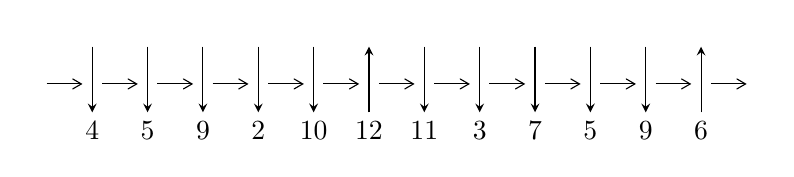
\begin{tikzpicture}[x=20pt, y=17pt]
	% nodes
	\node (C0) at (0, 0) {};
	\node (C1) at (1, 0) {};
	\node (C1U) at (1, +1) {};
	\node (C1D) at (1, -1) {4};

	\node (C2) at (2, 0) {};
	\node (C2U) at (2, +1) {};
	\node (C2D) at (2, -1) {5};

	\node (C3) at (3, 0) {};
	\node (C3U) at (3, +1) {};
	\node (C3D) at (3, -1) {9};

	\node (C4) at (4, 0) {};
	\node (C4U) at (4, +1) {};
	\node (C4D) at (4, -1) {2};

	\node (C5) at (5, 0) {};
	\node (C5U) at (5, +1) {};
	\node (C5D) at (5, -1) {10};

	\node (C6) at (6, 0) {};
	\node (C6U) at (6, +1) {};
	\node (C6D) at (6, -1) {12};

	\node (C7) at (7, 0) {};
	\node (C7U) at (7, +1) {};
	\node (C7D) at (7, -1) {11};

	\node (C8) at (8, 0) {};
	\node (C8U) at (8, +1) {};
	\node (C8D) at (8, -1) {3};

	\node (C9) at (9, 0) {};
	\node (C9U) at (9, +1) {};
	\node (C9D) at (9, -1) {7};

	\node (C10) at (10, 0) {};
	\node (C10U) at (10, +1) {};
	\node (C10D) at (10, -1) {5};

	\node (C11) at (11, 0) {};
	\node (C11U) at (11, +1) {};
	\node (C11D) at (11, -1) {9};

	\node (C12) at (12, 0) {};
	\node (C12U) at (12, +1) {};
	\node (C12D) at (12, -1) {6};
	\node (C13) at (13, 0) {};

	% arrows
	\draw[->,>={angle 60}]
	(C0) edge (C1) (C1) edge (C2) (C2) edge (C3) (C3) edge (C4) (C4) edge (C5) (C5) edge (C6) (C6) edge (C7) (C7) edge (C8) (C8) edge (C9) (C9) edge (C10) (C10) edge (C11) (C11) edge (C12) (C12) edge (C13) ;	\draw[->,>=stealth]
	(C1U) edge (C1D) (C2U) edge (C2D) (C3U) edge (C3D) (C4U) edge (C4D) (C5U) edge (C5D) (C6D) edge (C6U) (C7U) edge (C7D) (C8U) edge (C8D) (C9U) edge (C9D) (C10U) edge (C10D) (C11U) edge (C11D) (C12D) edge (C12U) ;
	\end{tikzpicture} \\
\hhline{~~} \\& 
\textbf{Solving Sequence} \\ \cline{2-2} 
 &
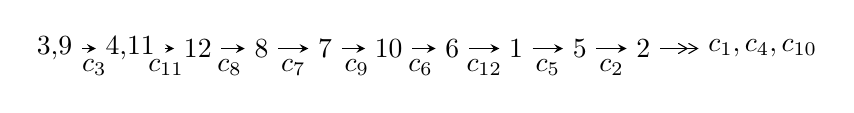
\begin{tikzpicture}[x=23pt, y=7pt]
	% node
	\node (A0) at (-1/8, 0) {3,9};
	\node (A1) at (17/16, 0) {4,11};
	\node (A2) at (17/8, 0) {12};
	\node (A3) at (25/8, 0) {8};
	\node (A4) at (33/8, 0) {7};
	\node (A5) at (41/8, 0) {10};
	\node (A6) at (49/8, 0) {6};
	\node (A7) at (57/8, 0) {1};
	\node (A8) at (65/8, 0) {5};
	\node (A9) at (73/8, 0) {2};
	\node (C1) at (1/2, -1) {$c_{3}$};
	\node (C2) at (13/8, -1) {$c_{11}$};
	\node (C3) at (21/8, -1) {$c_{8}$};
	\node (C4) at (29/8, -1) {$c_{7}$};
	\node (C5) at (37/8, -1) {$c_{9}$};
	\node (C6) at (45/8, -1) {$c_{6}$};
	\node (C7) at (53/8, -1) {$c_{12}$};
	\node (C8) at (61/8, -1) {$c_{5}$};
	\node (C9) at (69/8, -1) {$c_{2}$};
	\node (A10) at (11, 0) {$c_{1},c_{4},c_{10}$};

	% edge
	\draw[->,>=stealth]	
	(A0) edge (A1) (A1) edge (A2) (A2) edge (A3) (A3) edge (A4) (A4) edge (A5) (A5) edge (A6) (A6) edge (A7) (A7) edge (A8) (A8) edge (A9) ;
	\draw[->>,>={angle 60}]	
	(A9) edge (A10);
\end{tikzpicture} \\ 

\end{tabular} \\

\footnotetext{
The image of knot diagram is generated by the software ``\textbf{Draw programme}" developed by Andrew Bartholomew(\url{http://www.layer8.co.uk/maths/draw/index.htm\#Running-draw}), where we modified some parts for our purpose(\url{https://github.com/CATsTAILs/LinksPainter}).
}\phantom \\ \newline 
\centering \textbf{Ideals for irreducible components\footnotemark of $X_{\text{par}}$} 
 
\begin{align*}
I^u_{1}&=\langle 
-4.17337\times10^{102} u^{27}-1.93423\times10^{103} u^{26}+\cdots+3.84681\times10^{106} b+1.79302\times10^{107},\\
\phantom{I^u_{1}}&\phantom{= \langle  }-1.16409\times10^{103} u^{27}-5.28576\times10^{103} u^{26}+\cdots+7.69362\times10^{106} a+4.42452\times10^{107},\\
\phantom{I^u_{1}}&\phantom{= \langle  }u^{28}+4 u^{27}+\cdots-75264 u+25088\rangle \\
I^u_{2}&=\langle 
75504 u^{12}+165674 u^{11}+\cdots+485 b+93972,\;-42944 u^{12}-93489 u^{11}+\cdots+485 a-52132,\\
\phantom{I^u_{2}}&\phantom{= \langle  }u^{13}+3 u^{12}-3 u^{11}-4 u^{10}+u^9-5 u^8+12 u^7+23 u^6-15 u^5-13 u^4+12 u^3+u^2-3 u+1\rangle \\
\\
I^v_{1}&=\langle 
a,\;-579074 v^8-1101995 v^7+\cdots+5353327 b+7952402,\\
\phantom{I^v_{1}}&\phantom{= \langle  }v^9+v^8-8 v^7- v^6+33 v^5-23 v^4-14 v^3+2 v^2+3 v+7\rangle \\
\end{align*}
\raggedright * 3 irreducible components of $\dim_{\mathbb{C}}=0$, with total 50 representations.\\
\footnotetext{All coefficients of polynomials are rational numbers. But the coefficients are sometimes approximated in decimal forms when there is not enough margin.}
\newpage
\renewcommand{\arraystretch}{1}
\centering \section*{I. $I^u_{1}= \langle -4.17\times10^{102} u^{27}-1.93\times10^{103} u^{26}+\cdots+3.85\times10^{106} b+1.79\times10^{107},\;-1.16\times10^{103} u^{27}-5.29\times10^{103} u^{26}+\cdots+7.69\times10^{106} a+4.42\times10^{107},\;u^{28}+4 u^{27}+\cdots-75264 u+25088 \rangle$}
\flushleft \textbf{(i) Arc colorings}\\
\begin{tabular}{m{7pt} m{180pt} m{7pt} m{180pt} }
\flushright $a_{3}=$&$\begin{pmatrix}1\\0\end{pmatrix}$ \\
\flushright $a_{9}=$&$\begin{pmatrix}0\\u\end{pmatrix}$ \\
\flushright $a_{4}=$&$\begin{pmatrix}1\\u^2\end{pmatrix}$ \\
\flushright $a_{11}=$&$\begin{pmatrix}0.000151306 u^{27}+0.000687032 u^{26}+\cdots+8.22933 u-5.75089\\0.000108489 u^{27}+0.000502815 u^{26}+\cdots+7.32645 u-4.66105\end{pmatrix}$ \\
\flushright $a_{12}=$&$\begin{pmatrix}0.000151306 u^{27}+0.000687032 u^{26}+\cdots+8.22933 u-5.75089\\0.000150012 u^{27}+0.000689256 u^{26}+\cdots+9.68762 u-6.71343\end{pmatrix}$ \\
\flushright $a_{8}=$&$\begin{pmatrix}u\\u\end{pmatrix}$ \\
\flushright $a_{7}=$&$\begin{pmatrix}-0.0000766347 u^{27}-0.000357137 u^{26}+\cdots-1.56565 u+3.20147\\-0.0000700433 u^{27}-0.000319328 u^{26}+\cdots-3.53946 u+2.63866\end{pmatrix}$ \\
\flushright $a_{10}=$&$\begin{pmatrix}0.000123162 u^{27}+0.000561945 u^{26}+\cdots+8.07319 u-4.92967\\0.0000757763 u^{27}+0.000354447 u^{26}+\cdots+5.43594 u-3.01687\end{pmatrix}$ \\
\flushright $a_{6}=$&$\begin{pmatrix}-0.0000668361 u^{27}-0.000317419 u^{26}+\cdots-3.53613 u+1.93449\\0.0000195598 u^{27}+0.0000729436 u^{26}+\cdots+2.44504 u-1.73891\end{pmatrix}$ \\
\flushright $a_{1}=$&$\begin{pmatrix}0.0000318531 u^{27}+0.000142983 u^{26}+\cdots+1.78955 u-0.554362\\0.0000298229 u^{27}+0.000134348 u^{26}+\cdots+1.61686 u-1.48562\end{pmatrix}$ \\
\flushright $a_{5}=$&$\begin{pmatrix}-9.21121\times10^{-6} u^{27}-0.0000407445 u^{26}+\cdots-0.545453 u-0.540627\\0.0000226419 u^{27}+0.000102238 u^{26}+\cdots+1.24410 u-1.09499\end{pmatrix}$ \\
\flushright $a_{2}=$&$\begin{pmatrix}9.21121\times10^{-6} u^{27}+0.0000407445 u^{26}+\cdots+0.545453 u+0.540627\\0.0000242016 u^{27}+0.000109392 u^{26}+\cdots+1.30651 u-1.19282\end{pmatrix}$\\&\end{tabular}
\flushleft \textbf{(ii) Obstruction class $= -1$}\\~\\
\flushleft \textbf{(iii) Cusp Shapes $= -0.000152878 u^{27}-0.000780946 u^{26}+\cdots-9.76931 u-4.69330$}\\~\\
\newpage\renewcommand{\arraystretch}{1}
\flushleft \textbf{(iv) u-Polynomials at the component}\newline \\
\begin{tabular}{m{50pt}|m{274pt}}
Crossings & \hspace{64pt}u-Polynomials at each crossing \\
\hline $$\begin{aligned}c_{1},c_{2},c_{4}\end{aligned}$$&$\begin{aligned}
&u^{28}-16 u^{27}+\cdots+419 u-49
\end{aligned}$\\
\hline $$\begin{aligned}c_{3},c_{8}\end{aligned}$$&$\begin{aligned}
&u^{28}+4 u^{27}+\cdots-75264 u+25088
\end{aligned}$\\
\hline $$\begin{aligned}c_{5},c_{10}\end{aligned}$$&$\begin{aligned}
&u^{28}+2 u^{27}+\cdots-1173 u-1219
\end{aligned}$\\
\hline $$\begin{aligned}c_{6},c_{12}\end{aligned}$$&$\begin{aligned}
&u^{28}+3 u^{27}+\cdots+300 u+59
\end{aligned}$\\
\hline $$\begin{aligned}c_{7}\end{aligned}$$&$\begin{aligned}
&u^{28}- u^{27}+\cdots-246402 u-218849
\end{aligned}$\\
\hline $$\begin{aligned}c_{9}\end{aligned}$$&$\begin{aligned}
&u^{28}-4 u^{27}+\cdots+9 u-9
\end{aligned}$\\
\hline $$\begin{aligned}c_{11}\end{aligned}$$&$\begin{aligned}
&u^{28}- u^{27}+\cdots+26513 u+36713
\end{aligned}$\\
\hline
\end{tabular}\\~\\
\newpage\renewcommand{\arraystretch}{1}
\flushleft \textbf{(v) Riley Polynomials at the component}\newline \\
\begin{tabular}{m{50pt}|m{274pt}}
Crossings & \hspace{64pt}Riley Polynomials at each crossing \\
\hline $$\begin{aligned}c_{1},c_{2},c_{4}\end{aligned}$$&$\begin{aligned}
&y^{28}-4 y^{27}+\cdots-168113 y+2401
\end{aligned}$\\
\hline $$\begin{aligned}c_{3},c_{8}\end{aligned}$$&$\begin{aligned}
&y^{28}+78 y^{27}+\cdots+603717632 y+629407744
\end{aligned}$\\
\hline $$\begin{aligned}c_{5},c_{10}\end{aligned}$$&$\begin{aligned}
&y^{28}+42 y^{27}+\cdots+5986831 y+1485961
\end{aligned}$\\
\hline $$\begin{aligned}c_{6},c_{12}\end{aligned}$$&$\begin{aligned}
&y^{28}+y^{27}+\cdots-86696 y+3481
\end{aligned}$\\
\hline $$\begin{aligned}c_{7}\end{aligned}$$&$\begin{aligned}
&y^{28}+53 y^{27}+\cdots+367398468196 y+47894884801
\end{aligned}$\\
\hline $$\begin{aligned}c_{9}\end{aligned}$$&$\begin{aligned}
&y^{28}+2 y^{27}+\cdots-657 y+81
\end{aligned}$\\
\hline $$\begin{aligned}c_{11}\end{aligned}$$&$\begin{aligned}
&y^{28}+29 y^{27}+\cdots-4800844229 y+1347844369
\end{aligned}$\\
\hline
\end{tabular}\\~\\
\newpage\flushleft \textbf{(vi) Complex Volumes and Cusp Shapes}
$$\begin{array}{c|c|c}  
\text{Solutions to }I^u_{1}& \I (\text{vol} + \sqrt{-1}CS) & \text{Cusp shape}\\
 \hline 
\begin{aligned}
u &= \phantom{-}0.661495 + 0.747398 I \\
a &= -1.193220 + 0.182648 I \\
b &= -2.37661 + 0.83239 I\end{aligned}
 & -2.93456 - 1.71766 I & -11.35116 + 2.24777 I \\ \hline\begin{aligned}
u &= \phantom{-}0.661495 - 0.747398 I \\
a &= -1.193220 - 0.182648 I \\
b &= -2.37661 - 0.83239 I\end{aligned}
 & -2.93456 + 1.71766 I & -11.35116 - 2.24777 I \\ \hline\begin{aligned}
u &= -0.893984 + 0.439919 I \\
a &= \phantom{-}0.046736 - 0.846720 I \\
b &= -0.140462 - 0.488416 I\end{aligned}
 & -0.665833 - 0.463592 I & -8.88124 - 0.80143 I \\ \hline\begin{aligned}
u &= -0.893984 - 0.439919 I \\
a &= \phantom{-}0.046736 + 0.846720 I \\
b &= -0.140462 + 0.488416 I\end{aligned}
 & -0.665833 + 0.463592 I & -8.88124 + 0.80143 I \\ \hline\begin{aligned}
u &= -0.060146 + 1.078200 I \\
a &= -0.366791 - 0.845658 I \\
b &= -0.469643 + 0.590527 I\end{aligned}
 & \phantom{-}1.30627 + 3.65816 I & \phantom{-}0.62607 - 9.21590 I \\ \hline\begin{aligned}
u &= -0.060146 - 1.078200 I \\
a &= -0.366791 + 0.845658 I \\
b &= -0.469643 - 0.590527 I\end{aligned}
 & \phantom{-}1.30627 - 3.65816 I & \phantom{-}0.62607 + 9.21590 I \\ \hline\begin{aligned}
u &= \phantom{-}1.083710 + 0.326182 I \\
a &= \phantom{-}0.715235 - 0.997232 I \\
b &= \phantom{-}0.204712 + 0.075027 I\end{aligned}
 & -5.85717 + 6.56767 I & -13.7398 - 3.9298 I \\ \hline\begin{aligned}
u &= \phantom{-}1.083710 - 0.326182 I \\
a &= \phantom{-}0.715235 + 0.997232 I \\
b &= \phantom{-}0.204712 - 0.075027 I\end{aligned}
 & -5.85717 - 6.56767 I & -13.7398 + 3.9298 I \\ \hline\begin{aligned}
u &= -0.775820 + 0.972482 I \\
a &= \phantom{-}0.469871 + 0.774727 I \\
b &= -0.205034 - 0.207127 I\end{aligned}
 & -5.97045 + 2.54425 I & -12.99283 - 2.62358 I \\ \hline\begin{aligned}
u &= -0.775820 - 0.972482 I \\
a &= \phantom{-}0.469871 - 0.774727 I \\
b &= -0.205034 + 0.207127 I\end{aligned}
 & -5.97045 - 2.54425 I & -12.99283 + 2.62358 I\\
 \hline 
 \end{array}$$\newpage$$\begin{array}{c|c|c}  
\text{Solutions to }I^u_{1}& \I (\text{vol} + \sqrt{-1}CS) & \text{Cusp shape}\\
 \hline 
\begin{aligned}
u &= \phantom{-}0.617923 + 0.406438 I \\
a &= \phantom{-}1.204910 - 0.100272 I \\
b &= \phantom{-}0.612974 - 0.582117 I\end{aligned}
 & \phantom{-}2.45728 - 1.44782 I & -2.14877 + 4.95256 I \\ \hline\begin{aligned}
u &= \phantom{-}0.617923 - 0.406438 I \\
a &= \phantom{-}1.204910 + 0.100272 I \\
b &= \phantom{-}0.612974 + 0.582117 I\end{aligned}
 & \phantom{-}2.45728 + 1.44782 I & -2.14877 - 4.95256 I \\ \hline\begin{aligned}
u &= \phantom{-}0.585624 + 0.073997 I \\
a &= -0.95222 + 1.58256 I \\
b &= \phantom{-}0.16008 + 1.49787 I\end{aligned}
 & -2.72280 + 3.22335 I & -17.5168 - 5.4562 I \\ \hline\begin{aligned}
u &= \phantom{-}0.585624 - 0.073997 I \\
a &= -0.95222 - 1.58256 I \\
b &= \phantom{-}0.16008 - 1.49787 I\end{aligned}
 & -2.72280 - 3.22335 I & -17.5168 + 5.4562 I \\ \hline\begin{aligned}
u &= -0.528658\phantom{ +0.000000I} \\
a &= \phantom{-}0.651300\phantom{ +0.000000I} \\
b &= -0.226944\phantom{ +0.000000I}\end{aligned}
 & -0.770752\phantom{ +0.000000I} & -12.6200\phantom{ +0.000000I} \\ \hline\begin{aligned}
u &= -0.034927 + 0.413671 I \\
a &= \phantom{-}1.289190 - 0.171430 I \\
b &= -0.662191 + 0.707353 I\end{aligned}
 & -0.83719 + 2.37006 I & -4.55412 - 1.61124 I \\ \hline\begin{aligned}
u &= -0.034927 - 0.413671 I \\
a &= \phantom{-}1.289190 + 0.171430 I \\
b &= -0.662191 - 0.707353 I\end{aligned}
 & -0.83719 - 2.37006 I & -4.55412 + 1.61124 I \\ \hline\begin{aligned}
u &= \phantom{-}1.45117 + 2.14148 I \\
a &= -0.665316 - 0.045728 I \\
b &= -1.79657 + 0.17540 I\end{aligned}
 & \phantom{-}13.0799 - 5.8001 I & \phantom{-0.000000 } 0 \\ \hline\begin{aligned}
u &= \phantom{-}1.45117 - 2.14148 I \\
a &= -0.665316 + 0.045728 I \\
b &= -1.79657 - 0.17540 I\end{aligned}
 & \phantom{-}13.0799 + 5.8001 I & \phantom{-0.000000 } 0 \\ \hline\begin{aligned}
u &= -1.61598 + 2.05576 I \\
a &= -0.921601 - 0.257100 I \\
b &= -2.10745 - 0.14996 I\end{aligned}
 & \phantom{-}12.8917 + 14.5389 I & \phantom{-0.000000 } 0\\
 \hline 
 \end{array}$$\newpage$$\begin{array}{c|c|c}  
\text{Solutions to }I^u_{1}& \I (\text{vol} + \sqrt{-1}CS) & \text{Cusp shape}\\
 \hline 
\begin{aligned}
u &= -1.61598 - 2.05576 I \\
a &= -0.921601 + 0.257100 I \\
b &= -2.10745 + 0.14996 I\end{aligned}
 & \phantom{-}12.8917 - 14.5389 I & \phantom{-0.000000 } 0 \\ \hline\begin{aligned}
u &= \phantom{-}0.68402 + 3.16013 I \\
a &= \phantom{-}0.685728 - 0.115457 I \\
b &= \phantom{-}2.03515 - 0.07059 I\end{aligned}
 & \phantom{-}14.7956 - 5.0968 I & \phantom{-0.000000 } 0 \\ \hline\begin{aligned}
u &= \phantom{-}0.68402 - 3.16013 I \\
a &= \phantom{-}0.685728 + 0.115457 I \\
b &= \phantom{-}2.03515 + 0.07059 I\end{aligned}
 & \phantom{-}14.7956 + 5.0968 I & \phantom{-0.000000 } 0 \\ \hline\begin{aligned}
u &= -3.30423\phantom{ +0.000000I} \\
a &= \phantom{-}1.48289\phantom{ +0.000000I} \\
b &= \phantom{-}2.19015\phantom{ +0.000000I}\end{aligned}
 & -19.0273\phantom{ +0.000000I} & \phantom{-0.000000 } 0 \\ \hline\begin{aligned}
u &= -2.12239 + 3.48864 I \\
a &= -0.683688 + 0.783505 I \\
b &= -1.298960 + 0.127397 I\end{aligned}
 & \phantom{-}4.30987 - 2.62944 I & \phantom{-0.000000 } 0 \\ \hline\begin{aligned}
u &= -2.12239 - 3.48864 I \\
a &= -0.683688 - 0.783505 I \\
b &= -1.298960 - 0.127397 I\end{aligned}
 & \phantom{-}4.30987 + 2.62944 I & \phantom{-0.000000 } 0 \\ \hline\begin{aligned}
u &= \phantom{-}0.33576 + 4.88530 I \\
a &= \phantom{-}0.804068 - 0.346474 I \\
b &= \phantom{-}1.84810 + 0.02973 I\end{aligned}
 & \phantom{-}16.2350 - 2.8419 I & \phantom{-0.000000 } 0 \\ \hline\begin{aligned}
u &= \phantom{-}0.33576 - 4.88530 I \\
a &= \phantom{-}0.804068 + 0.346474 I \\
b &= \phantom{-}1.84810 - 0.02973 I\end{aligned}
 & \phantom{-}16.2350 + 2.8419 I & \phantom{-0.000000 } 0\\
 \hline 
 \end{array}$$\newpage\newpage\renewcommand{\arraystretch}{1}
\centering \section*{II. $I^u_{2}= \langle 75504 u^{12}+165674 u^{11}+\cdots+485 b+93972,\;-42944 u^{12}-93489 u^{11}+\cdots+485 a-52132,\;u^{13}+3 u^{12}+\cdots-3 u+1 \rangle$}
\flushleft \textbf{(i) Arc colorings}\\
\begin{tabular}{m{7pt} m{180pt} m{7pt} m{180pt} }
\flushright $a_{3}=$&$\begin{pmatrix}1\\0\end{pmatrix}$ \\
\flushright $a_{9}=$&$\begin{pmatrix}0\\u\end{pmatrix}$ \\
\flushright $a_{4}=$&$\begin{pmatrix}1\\u^2\end{pmatrix}$ \\
\flushright $a_{11}=$&$\begin{pmatrix}88.5443 u^{12}+192.761 u^{11}+\cdots-461.643 u+107.489\\-155.678 u^{12}-341.596 u^{11}+\cdots+801.984 u-193.757\end{pmatrix}$ \\
\flushright $a_{12}=$&$\begin{pmatrix}88.5443 u^{12}+192.761 u^{11}+\cdots-461.643 u+107.489\\-96.5423 u^{12}-212.656 u^{11}+\cdots+494.823 u-120.885\end{pmatrix}$ \\
\flushright $a_{8}=$&$\begin{pmatrix}u\\u\end{pmatrix}$ \\
\flushright $a_{7}=$&$\begin{pmatrix}308.078 u^{12}+670.996 u^{11}+\cdots-1605.18 u+378.957\\381.951 u^{12}+833.476 u^{11}+\cdots-1976.31 u+464.501\end{pmatrix}$ \\
\flushright $a_{10}=$&$\begin{pmatrix}-116.975 u^{12}-255.738 u^{11}+\cdots+606.153 u-145.751\\-361.198 u^{12}-790.095 u^{11}+\cdots+1870.78 u-446.996\end{pmatrix}$ \\
\flushright $a_{6}=$&$\begin{pmatrix}552.301 u^{12}+1205.35 u^{11}+\cdots-2868.81 u+680.202\\803.901 u^{12}+1754.95 u^{11}+\cdots-4169.61 u+986.002\end{pmatrix}$ \\
\flushright $a_{1}=$&$\begin{pmatrix}120.435 u^{12}+262.188 u^{11}+\cdots-628.151 u+148.470\\168.903 u^{12}+368.058 u^{11}+\cdots-879.431 u+207.606\end{pmatrix}$ \\
\flushright $a_{5}=$&$\begin{pmatrix}31.8907 u^{12}+69.4268 u^{11}+\cdots-166.507 u+39.9814\\-88.5443 u^{12}-192.761 u^{11}+\cdots+461.643 u-108.489\end{pmatrix}$ \\
\flushright $a_{2}=$&$\begin{pmatrix}31.8907 u^{12}+69.4268 u^{11}+\cdots-166.507 u+39.9814\\109.767 u^{12}+239.118 u^{11}+\cdots-572.270 u+134.734\end{pmatrix}$\\&\end{tabular}
\flushleft \textbf{(ii) Obstruction class $= 1$}\\~\\
\flushleft \textbf{(iii) Cusp Shapes $= \frac{296049}{485} u^{12}+\frac{650349}{485} u^{11}+\cdots-\frac{1491522}{485} u+\frac{340092}{485}$}\\~\\
\newpage\renewcommand{\arraystretch}{1}
\flushleft \textbf{(iv) u-Polynomials at the component}\newline \\
\begin{tabular}{m{50pt}|m{274pt}}
Crossings & \hspace{64pt}u-Polynomials at each crossing \\
\hline $$\begin{aligned}c_{1},c_{2}\end{aligned}$$&$\begin{aligned}
&u^{13}+6 u^{12}+\cdots-3 u+1
\end{aligned}$\\
\hline $$\begin{aligned}c_{3}\end{aligned}$$&$\begin{aligned}
&u^{13}+3 u^{12}+\cdots-3 u+1
\end{aligned}$\\
\hline $$\begin{aligned}c_{4}\end{aligned}$$&$\begin{aligned}
&u^{13}-6 u^{12}+\cdots-3 u-1
\end{aligned}$\\
\hline $$\begin{aligned}c_{5}\end{aligned}$$&$\begin{aligned}
&u^{13}+3 u^{11}+\cdots-3 u-1
\end{aligned}$\\
\hline $$\begin{aligned}c_{6}\end{aligned}$$&$\begin{aligned}
&u^{13}-3 u^{12}+\cdots+3 u^2+1
\end{aligned}$\\
\hline $$\begin{aligned}c_{7}\end{aligned}$$&$\begin{aligned}
&u^{13}-3 u^{12}+\cdots-6 u+1
\end{aligned}$\\
\hline $$\begin{aligned}c_{8}\end{aligned}$$&$\begin{aligned}
&u^{13}-3 u^{12}+\cdots-3 u-1
\end{aligned}$\\
\hline $$\begin{aligned}c_{9}\end{aligned}$$&$\begin{aligned}
&u^{13}+6 u^{12}+\cdots-3 u-1
\end{aligned}$\\
\hline $$\begin{aligned}c_{10}\end{aligned}$$&$\begin{aligned}
&u^{13}+3 u^{11}+\cdots-3 u+1
\end{aligned}$\\
\hline $$\begin{aligned}c_{11}\end{aligned}$$&$\begin{aligned}
&u^{13}+7 u^{12}+\cdots+5 u+1
\end{aligned}$\\
\hline $$\begin{aligned}c_{12}\end{aligned}$$&$\begin{aligned}
&u^{13}+3 u^{12}+\cdots-3 u^2-1
\end{aligned}$\\
\hline
\end{tabular}\\~\\
\newpage\renewcommand{\arraystretch}{1}
\flushleft \textbf{(v) Riley Polynomials at the component}\newline \\
\begin{tabular}{m{50pt}|m{274pt}}
Crossings & \hspace{64pt}Riley Polynomials at each crossing \\
\hline $$\begin{aligned}c_{1},c_{2},c_{4}\end{aligned}$$&$\begin{aligned}
&y^{13}-16 y^{12}+\cdots- y-1
\end{aligned}$\\
\hline $$\begin{aligned}c_{3},c_{8}\end{aligned}$$&$\begin{aligned}
&y^{13}-15 y^{12}+\cdots+7 y-1
\end{aligned}$\\
\hline $$\begin{aligned}c_{5},c_{10}\end{aligned}$$&$\begin{aligned}
&y^{13}+6 y^{12}+\cdots-5 y-1
\end{aligned}$\\
\hline $$\begin{aligned}c_{6},c_{12}\end{aligned}$$&$\begin{aligned}
&y^{13}+5 y^{12}+\cdots-6 y-1
\end{aligned}$\\
\hline $$\begin{aligned}c_{7}\end{aligned}$$&$\begin{aligned}
&y^{13}-15 y^{12}+\cdots+2 y-1
\end{aligned}$\\
\hline $$\begin{aligned}c_{9}\end{aligned}$$&$\begin{aligned}
&y^{13}-2 y^{12}+\cdots+15 y-1
\end{aligned}$\\
\hline $$\begin{aligned}c_{11}\end{aligned}$$&$\begin{aligned}
&y^{13}-31 y^{12}+\cdots+3 y-1
\end{aligned}$\\
\hline
\end{tabular}\\~\\
\newpage\flushleft \textbf{(vi) Complex Volumes and Cusp Shapes}
$$\begin{array}{c|c|c}  
\text{Solutions to }I^u_{2}& \I (\text{vol} + \sqrt{-1}CS) & \text{Cusp shape}\\
 \hline 
\begin{aligned}
u &= -0.816041 + 0.000203 I \\
a &= -1.61968 + 0.39099 I \\
b &= -1.80223 - 0.68201 I\end{aligned}
 & \phantom{-}1.72418 + 0.65957 I & -8.99705 + 2.64502 I \\ \hline\begin{aligned}
u &= -0.816041 - 0.000203 I \\
a &= -1.61968 - 0.39099 I \\
b &= -1.80223 + 0.68201 I\end{aligned}
 & \phantom{-}1.72418 - 0.65957 I & -8.99705 - 2.64502 I \\ \hline\begin{aligned}
u &= -1.128350 + 0.374297 I \\
a &= \phantom{-}0.383878 - 0.179213 I \\
b &= \phantom{-}0.067884 - 0.564804 I\end{aligned}
 & -6.59749 + 5.36054 I & -16.7957 - 3.3098 I \\ \hline\begin{aligned}
u &= -1.128350 - 0.374297 I \\
a &= \phantom{-}0.383878 + 0.179213 I \\
b &= \phantom{-}0.067884 + 0.564804 I\end{aligned}
 & -6.59749 - 5.36054 I & -16.7957 + 3.3098 I \\ \hline\begin{aligned}
u &= \phantom{-}0.556612 + 0.262804 I \\
a &= -1.195460 - 0.299951 I \\
b &= -0.22686 - 1.50683 I\end{aligned}
 & -1.55737 - 3.31191 I & -8.81382 + 5.67289 I \\ \hline\begin{aligned}
u &= \phantom{-}0.556612 - 0.262804 I \\
a &= -1.195460 + 0.299951 I \\
b &= -0.22686 + 1.50683 I\end{aligned}
 & -1.55737 + 3.31191 I & -8.81382 - 5.67289 I \\ \hline\begin{aligned}
u &= \phantom{-}1.312050 + 0.498669 I \\
a &= \phantom{-}0.473709 + 0.239750 I \\
b &= \phantom{-}0.594861 - 0.162148 I\end{aligned}
 & -4.99110 - 3.58519 I & -10.54784 + 4.86342 I \\ \hline\begin{aligned}
u &= \phantom{-}1.312050 - 0.498669 I \\
a &= \phantom{-}0.473709 - 0.239750 I \\
b &= \phantom{-}0.594861 + 0.162148 I\end{aligned}
 & -4.99110 + 3.58519 I & -10.54784 - 4.86342 I \\ \hline\begin{aligned}
u &= -0.00605 + 1.41713 I \\
a &= -0.242443 + 0.861161 I \\
b &= -0.561264 - 0.496045 I\end{aligned}
 & \phantom{-}0.87702 - 3.30359 I & -11.32603 - 0.21831 I \\ \hline\begin{aligned}
u &= -0.00605 - 1.41713 I \\
a &= -0.242443 - 0.861161 I \\
b &= -0.561264 + 0.496045 I\end{aligned}
 & \phantom{-}0.87702 + 3.30359 I & -11.32603 + 0.21831 I\\
 \hline 
 \end{array}$$\newpage$$\begin{array}{c|c|c}  
\text{Solutions to }I^u_{2}& \I (\text{vol} + \sqrt{-1}CS) & \text{Cusp shape}\\
 \hline 
\begin{aligned}
u &= \phantom{-}0.314233 + 0.325307 I \\
a &= -2.01758 + 0.09750 I \\
b &= -3.15000 + 2.21154 I\end{aligned}
 & -3.04698 - 2.63834 I & -10.8062 + 21.0195 I \\ \hline\begin{aligned}
u &= \phantom{-}0.314233 - 0.325307 I \\
a &= -2.01758 - 0.09750 I \\
b &= -3.15000 - 2.21154 I\end{aligned}
 & -3.04698 + 2.63834 I & -10.8062 - 21.0195 I \\ \hline\begin{aligned}
u &= -3.46490\phantom{ +0.000000I} \\
a &= \phantom{-}1.43517\phantom{ +0.000000I} \\
b &= \phantom{-}2.15521\phantom{ +0.000000I}\end{aligned}
 & -18.8747\phantom{ +0.000000I} & \phantom{-}13.5730\phantom{ +0.000000I}\\
 \hline 
 \end{array}$$\newpage\newpage\renewcommand{\arraystretch}{1}
\centering \section*{III. $I^v_{1}= \langle a,\;-5.79\times10^{5} v^{8}-1.10\times10^{6} v^{7}+\cdots+5.35\times10^{6} b+7.95\times10^{6},\;v^9+v^8+\cdots+3 v+7 \rangle$}
\flushleft \textbf{(i) Arc colorings}\\
\begin{tabular}{m{7pt} m{180pt} m{7pt} m{180pt} }
\flushright $a_{3}=$&$\begin{pmatrix}1\\0\end{pmatrix}$ \\
\flushright $a_{9}=$&$\begin{pmatrix}v\\0\end{pmatrix}$ \\
\flushright $a_{4}=$&$\begin{pmatrix}1\\0\end{pmatrix}$ \\
\flushright $a_{11}=$&$\begin{pmatrix}0\\0.108171 v^{8}+0.205852 v^{7}+\cdots-0.000774472 v-1.48551\end{pmatrix}$ \\
\flushright $a_{12}=$&$\begin{pmatrix}-0.102023 v^{8}-0.224509 v^{7}+\cdots+1.05024 v+0.683770\\0.108171 v^{8}+0.205852 v^{7}+\cdots-0.000774472 v-1.48551\end{pmatrix}$ \\
\flushright $a_{8}=$&$\begin{pmatrix}v\\0\end{pmatrix}$ \\
\flushright $a_{7}=$&$\begin{pmatrix}v\\0.109964 v^{8}+0.217820 v^{7}+\cdots-1.73167 v-1.00939\end{pmatrix}$ \\
\flushright $a_{10}=$&$\begin{pmatrix}0.159020 v^{8}+0.294157 v^{7}+\cdots-0.0933167 v-0.754991\\-0.0798487 v^{8}-0.139548 v^{7}+\cdots+0.391226 v-0.126428\end{pmatrix}$ \\
\flushright $a_{6}=$&$\begin{pmatrix}0.0944713 v^{8}+0.166302 v^{7}+\cdots+0.644723 v-0.337094\\0.0798487 v^{8}+0.139548 v^{7}+\cdots-0.391226 v+0.126428\end{pmatrix}$ \\
\flushright $a_{1}=$&$\begin{pmatrix}-0.163153 v^{8}-0.314762 v^{7}+\cdots+0.866612 v+1.49020\\-1\end{pmatrix}$ \\
\flushright $a_{5}=$&$\begin{pmatrix}0.163153 v^{8}+0.314762 v^{7}+\cdots-0.866612 v-1.49020\\1\end{pmatrix}$ \\
\flushright $a_{2}=$&$\begin{pmatrix}-0.163153 v^{8}-0.314762 v^{7}+\cdots+0.866612 v+2.49020\\-1\end{pmatrix}$\\&\end{tabular}
\flushleft \textbf{(ii) Obstruction class $= 1$}\\~\\
\flushleft \textbf{(iii) Cusp Shapes $= -\frac{37039389}{37473289} v^8-\frac{67980124}{37473289} v^7+\frac{235056117}{37473289} v^6+\frac{227362865}{37473289} v^5-\frac{992262694}{37473289} v^4+\frac{36681292}{37473289} v^3+\frac{60669880}{5353327} v^2+\frac{304560980}{37473289} v-\frac{262488239}{37473289}$}\\~\\
\newpage\renewcommand{\arraystretch}{1}
\flushleft \textbf{(iv) u-Polynomials at the component}\newline \\
\begin{tabular}{m{50pt}|m{274pt}}
Crossings & \hspace{64pt}u-Polynomials at each crossing \\
\hline $$\begin{aligned}c_{1},c_{2}\end{aligned}$$&$\begin{aligned}
&(u-1)^9
\end{aligned}$\\
\hline $$\begin{aligned}c_{3},c_{8}\end{aligned}$$&$\begin{aligned}
&u^9
\end{aligned}$\\
\hline $$\begin{aligned}c_{4}\end{aligned}$$&$\begin{aligned}
&(u+1)^9
\end{aligned}$\\
\hline $$\begin{aligned}c_{5}\end{aligned}$$&$\begin{aligned}
&u^9+u^8+2 u^7+u^6+3 u^5+u^4+2 u^3+u-1
\end{aligned}$\\
\hline $$\begin{aligned}c_{6}\end{aligned}$$&$\begin{aligned}
&u^9+3 u^8+8 u^7+13 u^6+17 u^5+17 u^4+12 u^3+6 u^2+u-1
\end{aligned}$\\
\hline $$\begin{aligned}c_{7}\end{aligned}$$&$\begin{aligned}
&u^9+u^8-2 u^7-3 u^6+u^5+3 u^4+2 u^3- u-1
\end{aligned}$\\
\hline $$\begin{aligned}c_{9}\end{aligned}$$&$\begin{aligned}
&u^9+5 u^8+12 u^7+15 u^6+9 u^5- u^4-4 u^3-2 u^2+u+1
\end{aligned}$\\
\hline $$\begin{aligned}c_{10}\end{aligned}$$&$\begin{aligned}
&u^9- u^8+2 u^7- u^6+3 u^5- u^4+2 u^3+u+1
\end{aligned}$\\
\hline $$\begin{aligned}c_{11}\end{aligned}$$&$\begin{aligned}
&u^9- u^8-2 u^7+3 u^6+u^5-3 u^4+2 u^3- u+1
\end{aligned}$\\
\hline $$\begin{aligned}c_{12}\end{aligned}$$&$\begin{aligned}
&u^9-3 u^8+8 u^7-13 u^6+17 u^5-17 u^4+12 u^3-6 u^2+u+1
\end{aligned}$\\
\hline
\end{tabular}\\~\\
\newpage\renewcommand{\arraystretch}{1}
\flushleft \textbf{(v) Riley Polynomials at the component}\newline \\
\begin{tabular}{m{50pt}|m{274pt}}
Crossings & \hspace{64pt}Riley Polynomials at each crossing \\
\hline $$\begin{aligned}c_{1},c_{2},c_{4}\end{aligned}$$&$\begin{aligned}
&(y-1)^9
\end{aligned}$\\
\hline $$\begin{aligned}c_{3},c_{8}\end{aligned}$$&$\begin{aligned}
&y^9
\end{aligned}$\\
\hline $$\begin{aligned}c_{5},c_{10}\end{aligned}$$&$\begin{aligned}
&y^9+3 y^8+8 y^7+13 y^6+17 y^5+17 y^4+12 y^3+6 y^2+y-1
\end{aligned}$\\
\hline $$\begin{aligned}c_{6},c_{12}\end{aligned}$$&$\begin{aligned}
&y^9+7 y^8+20 y^7+25 y^6+5 y^5-15 y^4+22 y^2+13 y-1
\end{aligned}$\\
\hline $$\begin{aligned}c_{7},c_{11}\end{aligned}$$&$\begin{aligned}
&y^9-5 y^8+12 y^7-15 y^6+9 y^5+y^4-4 y^3+2 y^2+y-1
\end{aligned}$\\
\hline $$\begin{aligned}c_{9}\end{aligned}$$&$\begin{aligned}
&y^9- y^8+12 y^7-7 y^6+37 y^5+y^4-10 y^2+5 y-1
\end{aligned}$\\
\hline
\end{tabular}\\~\\
\newpage\flushleft \textbf{(vi) Complex Volumes and Cusp Shapes}
$$\begin{array}{c|c|c}  
\text{Solutions to }I^v_{1}& \I (\text{vol} + \sqrt{-1}CS) & \text{Cusp shape}\\
 \hline 
\begin{aligned}
v &= \phantom{-}1.094310 + 0.114265 I \\
a &= \phantom{-0.000000 } 0 \\
b &= -0.650520 + 0.534295 I\end{aligned}
 & \phantom{-}0.13850 + 2.09337 I & -5.49232 - 4.08340 I \\ \hline\begin{aligned}
v &= \phantom{-}1.094310 - 0.114265 I \\
a &= \phantom{-0.000000 } 0 \\
b &= -0.650520 - 0.534295 I\end{aligned}
 & \phantom{-}0.13850 - 2.09337 I & -5.49232 + 4.08340 I \\ \hline\begin{aligned}
v &= -0.703774\phantom{ +0.000000I} \\
a &= \phantom{-0.000000 } 0 \\
b &= -1.17358\phantom{ +0.000000I}\end{aligned}
 & -2.84338\phantom{ +0.000000I} & -14.1380\phantom{ +0.000000I} \\ \hline\begin{aligned}
v &= -0.187998 + 0.564097 I \\
a &= \phantom{-0.000000 } 0 \\
b &= -1.104930 + 0.619057 I\end{aligned}
 & -2.26187 + 2.45442 I & -12.87375 - 1.42824 I \\ \hline\begin{aligned}
v &= -0.187998 - 0.564097 I \\
a &= \phantom{-0.000000 } 0 \\
b &= -1.104930 - 0.619057 I\end{aligned}
 & -2.26187 - 2.45442 I & -12.87375 + 1.42824 I \\ \hline\begin{aligned}
v &= \phantom{-}1.51733 + 0.93950 I \\
a &= \phantom{-0.000000 } 0 \\
b &= \phantom{-}0.443756 - 0.532821 I\end{aligned}
 & -6.01628 + 1.33617 I & -13.72452 + 1.86826 I \\ \hline\begin{aligned}
v &= \phantom{-}1.51733 - 0.93950 I \\
a &= \phantom{-0.000000 } 0 \\
b &= \phantom{-}0.443756 + 0.532821 I\end{aligned}
 & -6.01628 - 1.33617 I & -13.72452 - 1.86826 I \\ \hline\begin{aligned}
v &= -2.57175 + 0.82630 I \\
a &= \phantom{-0.000000 } 0 \\
b &= \phantom{-}0.469909 - 0.043588 I\end{aligned}
 & -5.24306 + 7.08493 I & -7.53426 - 10.08360 I \\ \hline\begin{aligned}
v &= -2.57175 - 0.82630 I \\
a &= \phantom{-0.000000 } 0 \\
b &= \phantom{-}0.469909 + 0.043588 I\end{aligned}
 & -5.24306 - 7.08493 I & -7.53426 + 10.08360 I\\
 \hline 
 \end{array}$$\newpage
\newpage\renewcommand{\arraystretch}{1}
\centering \section*{ IV. u-Polynomials}
\begin{tabular}{m{50pt}|m{274pt}}
Crossings & \hspace{64pt}u-Polynomials at each crossing \\
\hline $$\begin{aligned}c_{1},c_{2}\end{aligned}$$&$\begin{aligned}
&((u-1)^9)(u^{13}+6 u^{12}+\cdots-3 u+1)(u^{28}-16 u^{27}+\cdots+419 u-49)
\end{aligned}$\\
\hline $$\begin{aligned}c_{3}\end{aligned}$$&$\begin{aligned}
&u^9(u^{13}+3 u^{12}+\cdots-3 u+1)(u^{28}+4 u^{27}+\cdots-75264 u+25088)
\end{aligned}$\\
\hline $$\begin{aligned}c_{4}\end{aligned}$$&$\begin{aligned}
&((u+1)^9)(u^{13}-6 u^{12}+\cdots-3 u-1)(u^{28}-16 u^{27}+\cdots+419 u-49)
\end{aligned}$\\
\hline $$\begin{aligned}c_{5}\end{aligned}$$&$\begin{aligned}
&(u^9+u^8+\cdots+u-1)(u^{13}+3 u^{11}+\cdots-3 u-1)\\
&\cdot(u^{28}+2 u^{27}+\cdots-1173 u-1219)
\end{aligned}$\\
\hline $$\begin{aligned}c_{6}\end{aligned}$$&$\begin{aligned}
&(u^9+3 u^8+8 u^7+13 u^6+17 u^5+17 u^4+12 u^3+6 u^2+u-1)\\
&\cdot(u^{13}-3 u^{12}+\cdots+3 u^2+1)(u^{28}+3 u^{27}+\cdots+300 u+59)
\end{aligned}$\\
\hline $$\begin{aligned}c_{7}\end{aligned}$$&$\begin{aligned}
&(u^9+u^8+\cdots- u-1)(u^{13}-3 u^{12}+\cdots-6 u+1)\\
&\cdot(u^{28}- u^{27}+\cdots-246402 u-218849)
\end{aligned}$\\
\hline $$\begin{aligned}c_{8}\end{aligned}$$&$\begin{aligned}
&u^9(u^{13}-3 u^{12}+\cdots-3 u-1)(u^{28}+4 u^{27}+\cdots-75264 u+25088)
\end{aligned}$\\
\hline $$\begin{aligned}c_{9}\end{aligned}$$&$\begin{aligned}
&(u^9+5 u^8+12 u^7+15 u^6+9 u^5- u^4-4 u^3-2 u^2+u+1)\\
&\cdot(u^{13}+6 u^{12}+\cdots-3 u-1)(u^{28}-4 u^{27}+\cdots+9 u-9)
\end{aligned}$\\
\hline $$\begin{aligned}c_{10}\end{aligned}$$&$\begin{aligned}
&(u^9- u^8+\cdots+u+1)(u^{13}+3 u^{11}+\cdots-3 u+1)\\
&\cdot(u^{28}+2 u^{27}+\cdots-1173 u-1219)
\end{aligned}$\\
\hline $$\begin{aligned}c_{11}\end{aligned}$$&$\begin{aligned}
&(u^9- u^8+\cdots- u+1)(u^{13}+7 u^{12}+\cdots+5 u+1)\\
&\cdot(u^{28}- u^{27}+\cdots+26513 u+36713)
\end{aligned}$\\
\hline $$\begin{aligned}c_{12}\end{aligned}$$&$\begin{aligned}
&(u^9-3 u^8+8 u^7-13 u^6+17 u^5-17 u^4+12 u^3-6 u^2+u+1)\\
&\cdot(u^{13}+3 u^{12}+\cdots-3 u^2-1)(u^{28}+3 u^{27}+\cdots+300 u+59)
\end{aligned}$\\
\hline
\end{tabular}\newpage\renewcommand{\arraystretch}{1}
\centering \section*{ V. Riley Polynomials}
\begin{tabular}{m{50pt}|m{274pt}}
Crossings & \hspace{64pt}Riley Polynomials at each crossing \\
\hline $$\begin{aligned}c_{1},c_{2},c_{4}\end{aligned}$$&$\begin{aligned}
&((y-1)^9)(y^{13}-16 y^{12}+\cdots- y-1)\\
&\cdot(y^{28}-4 y^{27}+\cdots-168113 y+2401)
\end{aligned}$\\
\hline $$\begin{aligned}c_{3},c_{8}\end{aligned}$$&$\begin{aligned}
&y^9(y^{13}-15 y^{12}+\cdots+7 y-1)\\
&\cdot(y^{28}+78 y^{27}+\cdots+603717632 y+629407744)
\end{aligned}$\\
\hline $$\begin{aligned}c_{5},c_{10}\end{aligned}$$&$\begin{aligned}
&(y^9+3 y^8+8 y^7+13 y^6+17 y^5+17 y^4+12 y^3+6 y^2+y-1)\\
&\cdot(y^{13}+6 y^{12}+\cdots-5 y-1)(y^{28}+42 y^{27}+\cdots+5986831 y+1485961)
\end{aligned}$\\
\hline $$\begin{aligned}c_{6},c_{12}\end{aligned}$$&$\begin{aligned}
&(y^9+7 y^8+20 y^7+25 y^6+5 y^5-15 y^4+22 y^2+13 y-1)\\
&\cdot(y^{13}+5 y^{12}+\cdots-6 y-1)(y^{28}+y^{27}+\cdots-86696 y+3481)
\end{aligned}$\\
\hline $$\begin{aligned}c_{7}\end{aligned}$$&$\begin{aligned}
&(y^9-5 y^8+12 y^7-15 y^6+9 y^5+y^4-4 y^3+2 y^2+y-1)\\
&\cdot(y^{13}-15 y^{12}+\cdots+2 y-1)\\
&\cdot(y^{28}+53 y^{27}+\cdots+367398468196 y+47894884801)
\end{aligned}$\\
\hline $$\begin{aligned}c_{9}\end{aligned}$$&$\begin{aligned}
&(y^9- y^8+12 y^7-7 y^6+37 y^5+y^4-10 y^2+5 y-1)\\
&\cdot(y^{13}-2 y^{12}+\cdots+15 y-1)(y^{28}+2 y^{27}+\cdots-657 y+81)
\end{aligned}$\\
\hline $$\begin{aligned}c_{11}\end{aligned}$$&$\begin{aligned}
&(y^9-5 y^8+12 y^7-15 y^6+9 y^5+y^4-4 y^3+2 y^2+y-1)\\
&\cdot(y^{13}-31 y^{12}+\cdots+3 y-1)\\
&\cdot(y^{28}+29 y^{27}+\cdots-4800844229 y+1347844369)
\end{aligned}$\\
\hline
\end{tabular}
\vskip 2pc
\end{document}